\documentclass[a4paper]{ctexart}
\usepackage{geometry}
\usepackage{graphicx}
\usepackage{pstricks}
\usepackage{multicol}
\usepackage{pst-plot}
\geometry{left=2cm,right=2cm,top=2.5cm,bottom=2.5cm}

\author{严春伟\\ 1201213679}
\title{密码学个人作业}
\begin{document}
    \maketitle

\part{数字城市与网络信息安全}
    \section{数字城市发展概况}
    \par 数字城市是以计算机技术、多媒体技术和大规模存储技术为基础,以宽带网络为纽带,运用遥感、全球定位系统、地理信息系统、遥测、仿真-虚拟等技术,对城市进行多分辨率、多尺度、多时空和多种类的三维描述,即利用信息技术手段把城市的过去、现状和未来的全部内容在网络上进行数字化虚拟实现。 \cite{china-digital-city}

    \section{数字城市支撑技术}
    \subsection{遥感技术}
    \par 数字城市致力于将城市数字化建模.在城市数字化方面,遥感技术有很大的应用空间.
    \begin{enumerate}
        \item 拓展综合信息源. 现代城市中有极丰富的人文社会化信息,利用GIS和遥感集成技术将此方面信息整合起来,为宏观上探测城市的综合信息提供了技术可能.
        \item 动态变化. 遥感技术可以动态更新,实现数据实时性,趋势性的要求.
        \item 监测评估功能. 能够对城市资源,经济,人文实时监控. 通过反馈评估,使城市健康高效运行.
    \end{enumerate}

    \subsection{信息技术}
    \par 信息技术的发展能实现信息空间的扩展与城市空间的延伸.
    \begin{enumerate}
        \item 通过信息技术的支持,能集中城市经济规划与管理的职能,提供生产和消费市场的在线服务,消除信息互动的物质空间距离.
        \item 提供便利的城市社会文化生活,为市民提供相关的服务. 数字城市的管理中心能够便捷地与市民间实现便捷而方便的互动.
        \item 促进虚拟社区的发展. 强化了物质社区的功能,推动信息时代社区功能的全面复兴和发展.
    \end{enumerate}

    \subsection{网络技术}
    ``数字城市''涉及到大量图形、影像、视频等多媒体数据,数据量非常大,目前的因特网难以胜任,必须使用宽带网络。城市宽带网技术发展很快,据报道,国内已有城市开始建立每秒10G的宽带网络。这种宽带网络可以满足''数字城市''的需要。

    \section{数字城市中网络信息安全的必要性}
    \par 从数字城市的三个核心技术来看,信息系统和遥感技术等产生繁多的数据,而这些数据需要有强大而安全的存储系统,而相关信息的传输以及整合便需要安全有效的网络技术的支撑。
    \par 那么关于数字城市中繁杂而频繁的网络信息的传输,以及大数据的存储,均需要有强大的网络安全技术支撑。
    \par 近年来 发生在互联网上的安全事故频频发生,据 IT 界企业团体ITAA 的调查显示,目前美国约75 万的企业网的信息失窃,25万的企业损失高达25万美元以上。 由此,可以看到在信息安全比较脆弱环境下,数字城市所面临的安全挑战。 由于数字城市整个大系统中信息比较全面,如果相关信息泄露会威胁整个城市框架中很多的运行核心信息的安全。
    \par 一个典型的事例就是,城市中出现了一个劫持事件,那么在城市的管理中枢(指挥中心)会尝试整合数字城市中各方面丰富的信息进行分析,这些信息包括歹徒方向的,卫星、监控录像、通话等等信息;同时,也会包括警察这方面的部署、人员配置等等方面的信息。我们不能想象如果歹徒能够窃取这方面的信息,掌控了整个大局的后果。 如此,信息安全的重要性可见一斑。
    \par 在网络化信息化进程不可逆转的形势下如何最大限度地减少或避免因信息泄漏,破坏所造成的经 济损失 是摆在我们面前亟需妥善解决的一项具有重大战略意义的课题。 

    \section{中外安全技术支撑}
    \subsection{病毒防范技术}
\par 数字城市健康运行需要庞大规模的计算机群的运行。 如今,计算机病毒能够经过系统穿透或违反授权攻击成功在系统中植入木马或逻辑炸弹等程序,直接威胁到数字城市信息安全以及电子设施的稳健。
\par 因此,数字城市需要完善的病毒防范技术。
\par 在这些方面国外的一些杀毒软件如Norton McAfee 熊猫卫士等走在了前面,而国内的大部分杀毒软件大都专注在单机版杀毒上。虽然有部分厂商推出了网络版的杀毒产品,也只是在桌面端及文件服务器上进行防护,防护范围依然较窄。所以国内杀毒厂商应及早加强在网关或邮件服务器上的防护,只有有效截断病毒的入口,才能避免电子城市的电子设施遭受病毒侵害。 

    \subsection{加密型技术}
    \par 采用加密技术,能够保证电子城市的各职能部门间的信息安全。通过对网络数据的可靠加密来保护网络系统中包括用户数据在内的所有数据流,从而在不对网络环境作任何特殊要求的前提下,从根本上解决了网络安全的两大要求:即网络服务的可用性和信息的完整性。
    \par 加密技术可以分为对称加密、不对称加密以及不可逆加密,下面进行简单介绍。 
    对称型加密 使用单个密钥对数据进行加密或解密。这是比较传统的一种加密方法,发信人用密钥将某重要信息加密后,通过网络传给收信人,收信人再用同一密钥将加密后的信息解 密。这种方法的优点是计算量小加密效率高 即使传输信息的网络不安全,被别人截走信息加密后的信息也不易泄漏。

    \subsubsection{不对称型加密} 
    \par 其特点是有两个密钥 一个称为公用密钥 另一个称为私有密钥。其中公用密钥在网上公布,为数据源对数据加密使用, 而用于解密的相应私有密钥则由数据的收信方妥善保管。
    \par 由于秘钥的分拆,可以实现分布式的加密,在互联网中可以有很大的应用。

    \subsubsection{不可逆加密} 
    \par 这种加密的特征是加密过程不需要密钥,且经过加密后的数据无法被解密,只有同样的输入数据经过同样的不可逆加密,算法才能得到相同的加密数据。


    \begin{thebibliography}{sotief}
            \bibitem{china-digital-city} 王家耀,宁津生,张祖勋.中国数字城市建设方案及推进战略研究.北京:科学出版社.2008
            \bibitem{digital-technology}许奕锋,试论数字城市建设与管理的三大技术支撑,湖南省委党校,湖南长沙
            \bibitem{security-technology} 沈昌祥,张焕国,冯登国,曹珍富,黄继武. 信息安全综述 ,中国科学,2007
    \end{thebibliography}

%--- yunjisuan -----
    \part{云计算安全}
    \section{前言}
    \par 云计算是一种以网络为载体,整合大规模可扩展的服务形式。云计算能够将包括计算、存储、数据、应用等可扩展的,分布式资源高效分配和协同工作,从而实现一种超级计算模式。 
    \par 通过整合相关的资源提供更加由弹性的服务,以及集中式的,更加可靠中央服务,云计算可以说是一种相当成功的商业运行模式,在当今信息时代大行其道。但最着云计算的快速发展,云计算领域也面临着各种潜在的风险和安全隐患。 
    \par 本文将会阐述云计算安全方面的一些技术。 

    \section{云计算安全的挑战}
    \subsection{云安全的一些事故}
    云计算发展的这几年,已经发生了一些事故,这里总结了2012年前的大的事故
    \begin{itemize}
        \item 2008年2月15日Amazon出现了网络服务宕机事件,使得几千个依赖亚马逊的EC2云计算和s3云存储的网站受到影响
        \item 2009年2月24日,Google Gmail邮箱爆发全球性故障,服务中断时间长达4h,起因其一个数据中心例行维护,使得另外一个数据中心过载
        \item 2009年3月7日,Google发生大批用户文件外泄事件
        \item 2009年3月15日,Microsoft的云计算平台Azure停止运行长达22h
        \item 2009年6月11日,Amazon的EC2中断了几个小时,起因是雷击损坏了公司数据中心的电力设施
        \item 2010年1月,几乎6万8千名的Salesforce.com用户经历了至少1个小时的宕机。
        \item 2010年3月,VMware的合作伙伴Terremark就发生了七小时的停机事件
        \item 2011年3月,gmail再次爆发大规模的用户数据泄漏事件,大约有15万Gmail用户在周日早上发现自己的所有邮件和聊天记录被删除
        \item 2011年4月22日,亚马逊云数据中心服务器大面积宕机,这一事件被认为是亚马逊史上最为严重的云计算安全事件
    \end{itemize}
    {\color{red}
    总结这些事故,可以得到一些结论:
    \par 与传统的网络安全多针对软件漏洞不同,云计算安全事故涉及到软件和硬件两个方面。硬件方面,如停电、停机等事故,或者负荷超载等造成的宕机;软件方面,由于一些常规的软件安全方面的漏洞,造成用户的信息外泄,比如Gmail或者Microsoft的用户信息外泄
    \par 云计算框架把更多的计算资源整合成一个整体,但其中一个部分出现问题也会使整体的服务发生很大的影响。比如Gmail全球性的服务中断,仅因为欧洲的一个数据中心超载。
\par 由于云计算厂商同时服务着众多的用户,云计算服务短暂的事故也影响非常广泛。2010年1月著名的云计算厂商Salesforce.com 1个小时的宕机,影响了几乎6万 8千名云计算的用户。}

    \subsubsection{云计算五大问题}
    \begin{enumerate}
        \item 虚拟化安全问题
        \item 数据集中后的安全问题
        \item 云平台可用性问题
        \item 云平台遭受攻击问题
        \item 法律问题
    \end{enumerate}
    \section{云计算安全的关键技术}
        \subsection{数据安全}
        \subsubsection{数据传输安全}
            \par 在使用公共云时,数据加密至关重要。一般云计算服务商会对存储的数据进行加密,在数据传输的时候,采用SSL,SSH等安全协议保证安全访问。但是,还是有一个隐患,那就是在内存中的数据,依旧是明文,这为使得利用操作系统漏洞攻击载入内存中的数据成为可能。
        \subsubsection{数据隔离}
            \par 采用安全独立的云区域提供虚拟机来实现数据资源的高度隔离,除此以外,云服务商与组织内部的通信采用加密的VPN专用通道。

        \subsubsection{数据残留}
            {\color{red}
            \par 由于公共云中,共享资源高度重用,并被用户共享。当一个用户的数据空间被废弃,但是由于内存或者硬盘的物理特性可以被恢复数据,这就客观上残留了用户敏感数据泄露的可能。 因此,云计算服务商需要保证一个用户的数据空间在回收后,必须进行彻底的擦除后再分配给其他用户使用。 在应用中,相关技术已经比较成熟。

        \subsection{应用安全}
            \par 云计算安全的实质是安全责任的转移,云计算时代之前,由单个用户自己负责服务器的安全及维护,而如今,用户将自己的服务架设在云计算框架上,将一部分安全责任转嫁到自己信任的云计算服务提供商身上。 
            \par 将分散的小应用部署到“云”上,可以降低单个用户的运营维护的压力。例如:最近沸沸扬扬的12306订票网站(12月16日和9日,此网站因为空调故障两度瘫痪,影响的用户应该是千万级),如果架构在SAE(sina云计算平台)上,那么应该就不必要有这么多宕机事件(如果出问题,那么大部分责任是SAE的,远不是单纯12306本身的问题了)。另外,如果当初开发的时候就考虑到要部署到“云”上,那么此前的沸沸扬扬的9亿元升级其实只需要在SAE那边扩容而已,而且还可以在重要时段进行暂时性的扩容,以应对春节或者国庆长假时候的压力。但是是否足够信任 “云”上的运行安全,是一个考察决策者智慧和勇气的,在作者看来,如今的12306,除非从底层进行重构,或者部署到“云”上,否则所谓的升级只能是一条不归路。
        \par 就像能量守恒定律一样,安全责任不可能消失,只能通过转移的方式得到最优的效果。}

        \subsection{终端用户的安全}
            \par 对于管理远程“云”上应用的用户,自己所用计算机就像钥匙,钥匙丢了,那就算有最坚固的防盗门也是形同虚设。用户的账户信息的安全也需要用户自己多加保密,同时, 用户所用终端机器上也需要有完善的安全软件的保护。 用户需要注意自己所用终端软件的安全,比如浏览器的安全漏洞问题等,定期做好打补丁以及杀毒软件的更新,从终端角度确保云安全。

        \subsection{应用运维的安全}
            \par 应用在云平台的安全运行,当然,需要云计算服务提供端的高度配合。 如PaaS云提供商能够为用户提供相对安全的应用运行环境,也就是云计算服务提供商承担了运行安全相关的责任,通过一定的措施如虚拟化或者沙箱,保证应用运行时不会受到云架构内部或者外部的侵犯。
            \par {\color{red} 但应用本身的安全责任也需要考虑。 如果应用是用户自行开发,那么用户自己需要承担应用本身的安全责任,如果应用当中用到了第三方的程序,那么第三方需要承担自己程序部分的安全责任。}
            \par 目前PaaS服务提供商为了安全,会提供自行维护安全的平台API,比如很多安全特性被封装成了平台相关的安全对象和Web服务,用户的应用需要注意调用这些“云”上高效集成和安全的接口,能够更加高效地保证其运行的安全。
            \par 而IaaS云提供商的服务利用虚拟机来分隔应用,每个虚拟机相当于一个相对独立和部分完整功能的操作系统。把虚拟机当做为一个沙箱,IaaS提供商的服务并不能够穿透沙箱,因此虚拟机中运行的应用对于云提供商是完全透明的,用户需要自行负责自己应用的大部分安全维护以及其他责任。
            \par 用户自己需要有一定的安全运维的实力,这一方面IaaS云提供商并不会有太大的协助。

        \subsection{虚拟化安全}
        \par 基于虚拟化技术的云计算的安全主要有两方面:一是虚拟化软件的安全; 另外一个是使用虚拟化技术的虚拟服务器的安全。

        \subsubsection{虚拟软件安全}
            \par 该软件层直接部署在裸机之上,虚拟的主要是服务器。IaaS云平台上,该软件层对于用户是透明的,管理方面完全是云提供商的义务。
            \par 由于虚拟化软件层运行在多租户的环境下,一台主机也许被多个用户多个虚拟机分享。 云计算提供商会采取一定的措施,严格限制未授权的用户访问虚拟化软件层,限制对于Hypervisor和其他形式的虚拟化层次的物理和逻辑访问控制。

        \subsubsection{虚拟服务器安全}
            \par 应该选择具有TPM安全模块的物理服务器,TPM安全模块可以再虚拟服务器启动时,监测用户密码,如果发现密码及用户名的Hash序列不对,就不会启动此虚拟服务器。 尽可能使用新的带有多核的处理器,并支持虚拟技术的CPU,这就能保证CPU之间的物理隔离,提高安全性。
            \par 另外,为了实现各虚拟服务器间物理隔离的目的,应该在创建虚拟服务器的时候,为每一台虚拟机分配一个独立的分区,以实现磁盘页表的分隔。 每台虚拟机系统还需要安全自己独立的完整的安全防护系统,如防火墙、杀毒软件等。 另外,对于虚拟机的备份也非常重要,如数据、配置需要定期备份,以提供完整的增量或差量备份方式。

        \subsection{物理及其他方面的安全}
        \par 云计算是一种大量消耗硬件的服务方式,底层硬件的稳固以及各方面客观条件的支持对其稳定运行至关重要。
        \subsubsection{电力及其他设施}
        \par 对于云计算系统的稳固运行,电力系统首当其冲。可以看到,亚马逊的前几次故障均与电力有关。 电力的备份非常重要,因此,google的工程师甚至为每台主机配备了单独的蓄电池。
        \subsubsection{人员安全}
        \par 完整的商业道德以及职业操守对于在关键领域的公司员工非常重要,企业应该主动培养员工的责任意识。
        \par 同时,相关的安保措施也需要加强。 在网络虚拟的安全,也需要现实中的严格安保措施去保障。
        \subsubsection{冗余度和扩展性}
        \par 除了部分大企业会使用大型机和非常昂贵的高可用性解决方案来保证核心应用能达到5个9个的可用性,普通企业数据中心的冗余度还是有所欠缺的,就连非常专业的互联网企业也很难独善其生. 比如,2010年上半年国内某大型视频网站接连出现各种待机现象. 虽然现在也经常出现小事故,但是和一两年前相比,无聊从影响规模还是持续时间上,都得到了极大的改善.\cite{core-tech}
        \begin{thebibliography}{sotief}
                \bibitem{core-tech} 吴朱华,云计算核心技术剖析.人民邮电出版社.2011
        \end{thebibliography}
    \part{QQ 远程协助抓包及 360监控原理}
    \section{QQ远程协助抓包分析  }
        \begin{figure}[]
            \centering
            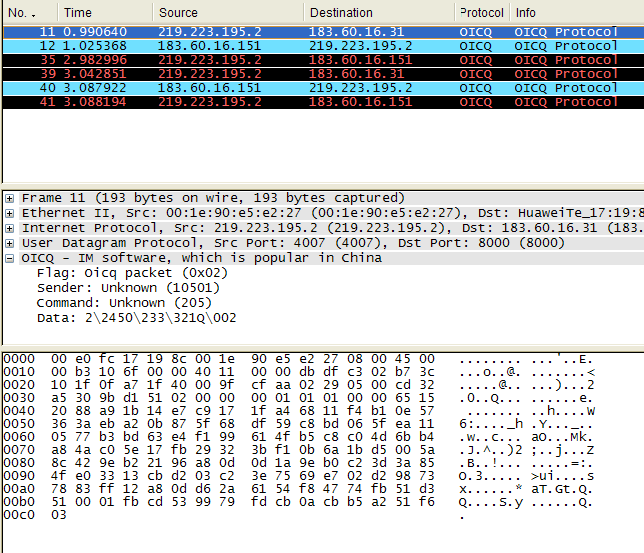
\includegraphics[width=400pt]{qq.png}
            \caption{协议抓包结果}
            \label{fig:qq}
        \end{figure}
\par 从抓包结果可以看到:
\par 本机IP为129.223.195.2
服务器IP有2个分别为:
    \par 183.60.16.31、183.60.16.151
    \par 可以看到,OICQ协议时基于UDP协议传输的,包括了类型,发送者,以及加密的数据。采用UDP传播是由于远程协助需要比较大的带宽来传播桌面的视频。而UDP很适合于突发性短期性的内容传播。
    \par 之前以为QQ的远程协助是完全通过UDP两个客户端之间的传播,但是,试验发现中间总是会有服务器插一脚。 当然如果是文本内容的话,中间服务器可以有保存历史信息以及关键词监控等功能。 但不清楚远程协助中央服务器需要监控什么。
    \section{360监控方法}
    \subsection{云查杀}
    \par 360推出的云查杀是360推出的一个能够与360杀毒软件协同工作的工具。 云查杀主要的优势是将杀毒软件的一部分功能移植到了云平台上,从而达到客户端瘦身的目标。采用云查杀的机器,不需要频繁升级木马库,而且运行速度也快很多。
    \par 云查杀的原理比较简单,把所有的病毒库和木马库都放在中央服务器集群上。大部分匹配和计算的工作都放在云端。在用户的电脑上,如果发现一个陌生的程序,就会被采集并传到中央服务器集群,如果这个程序产生传播行为,又传播到一个新的机器里面,这台机器也会向中央集群报告,当100、500、1000台机器报告了,中央云平台就会报警,同时将这个文件作为病毒加到中央病毒库中。 同时对所有的客户端发送警告,预防该恶意程序。 
    {\color{red}
    \par 但是,云查杀由于需要将用户机器上的一些文件甚至用户的使用行为记录远程上传到云端。因此很容易就会泄露用户隐私。同时,如果用户都选择对本机的文件不上传,那么360的所谓云查杀也就名存实亡。
    \par 360对于这些比较敏感的服务一直都是采取逃避或者诱导用户授权的方式。也有报道说,360的云查杀在没有用户授权的时候也默认打开,这无疑对360公司监控用户行为,窃取用户信息带来了N种可能。行业内普遍地不尊重用户隐私及权利的大氛围下,360作为一个安全公司,长久以来也偷偷地监控用户行为,这无疑让人失望。
}
    \subsection{360隐私保护器原理}
    \par 360隐私保护器可以监控其他程序对文件读取的过程。通过监控这些程序的文件操作过程,同时对特定的隐私文件重点防控,可以防止其他程序侵犯用户隐私。
    \par 360隐私保护器仅获取被保护文件的所在路径和文件名,不会涉及被保护文件包含的具体内容。
\end{document}

